\documentclass[12pt, a4paper]{report}

% \usepackage[french]{babel}
\usepackage[utf8]{inputenc} 
\usepackage{csquotes}
% \usepackage[T1]{fontenc}
\usepackage{array}
\usepackage{amsmath, amssymb, amsfonts, amsthm}
\usepackage{xcolor}
\usepackage{fancyhdr}
\usepackage{graphicx}
\usepackage{enumitem}
\usepackage{import}

\usepackage{hyperref}
\hypersetup{
    colorlinks=true,
    linkcolor=black,
	urlcolor=blue,
	citecolor=black,
}
\usepackage{geometry}
\graphicspath{{../assets/images/}}
\newlength\figureheight
\newlength\figurewidth

\usepackage[backend=biber]{biblatex}
\addbibresource{references.bib}

\usepackage{arabtex}
\usepackage{utf8}
\setcode{utf8}

\usepackage{listings}
\renewcommand\lstlistingname{Bloc de code}
\renewcommand\lstlistlistingname{Liste des blocs de code}
%Code zones styling
\definecolor{codegreen}{rgb}{0,0.6,0}
\definecolor{codegray}{rgb}{0.5,0.5,0.5}
\definecolor{codepurple}{rgb}{0.58,0,0.82}
\definecolor{backcolour}{rgb}{0.95,0.95,0.92}
\lstdefinestyle{mystyle}{
	backgroundcolor=\color{backcolour},   
	commentstyle=\color{codegreen},
	keywordstyle=\color{magenta},
	numberstyle=\tiny\color{codegray},
	stringstyle=\color{codepurple},
	basicstyle=\ttfamily\footnotesize,
	breakatwhitespace=false,         
	breaklines=true,                 
	captionpos=b,                    
	keepspaces=true,                 
	numbers=left,                    
	numbersep=5pt,                  
	showspaces=false,                
	showstringspaces=false,
	showtabs=false,                  
	tabsize=2
}
\lstset{style=mystyle}
\usepackage{afterpage}
\usepackage{float}
\usepackage{subfig}

\usepackage[inline]{asymptote}
\usepackage{tikz}
\usetikzlibrary{calc}

\setlength{\parskip}{.4cm}

\newtheorem{theorem}{Theorem}[chapter]
\newtheorem{lemma}{Leamma}
\newtheorem{corollary}{Corollary}[theorem]
\theoremstyle{definition}
\newtheorem{thedef}[theorem]{Theorem and definition}
\newtheorem{definition}{Definition}
\newtheorem{example}{Example}[chapter]
\theoremstyle{remark}
\newtheorem{remark}{Remark}

% Definition of number sets
\newcommand{\complexes}{\mathbb{C}}
\newcommand{\reals}{\mathbb{R}}
\newcommand{\rationals}{\mathbb{Q}}
\newcommand{\integers}{\mathbb{Z}}
\newcommand{\naturals}{\mathbb{N}}
\newcommand{\field}{\mathbb{K}}

\author{Mohammed D. Belgoumri}
\title{
	{
		\bfseries
		\Huge
		My notes while reading:\\

		\Large
		An Introduction To Computational Learning Theory

	}
}

\date{\today}
%!TEX root = main.tex
\begin{document}
	% \makeatletter

\begin{titlepage}
    \pagecolor{blue!20}
    \centering
    
    \ \\
    \Large
    \vspace{5cm}

    My notes while reading:

    \vspace{2cm}
    \hrulefill
    {
        \Huge
        {
            \bfseries

            \@title
        }
    }

    \hrulefill
    \vspace{2cm}
    
    \@author

    \vfill
    
    \@date
\end{titlepage}
	\maketitle
	\addcontentsline{toc}{chapter}{Title page}
	\tableofcontents
	\chapter{The Probably Approximately Correct Learning Model}
    \section{A Rectangle Learning Game}
\newcommand{\rectangle}{\mathcal{R}}
The objective of this game is to learn an unknown \emph{target} (axis-aligned) rectangle \(\rectangle = [a, b] \times [c, d] \subset \reals^2\).

The player can gain information about \(\rectangle\) only by chosing random points according to some distribution \(\mathcal{D}\), and asking the game whether they are inside \(\rectangle\). By convention, points inside \(\rectangle\) are considered positive.

Figure~\ref{fig:traget-and-sample} shows an example of a possible target rectangle \(\rectangle\) along with some points labeled using it.

\begin{figure}
    \begin{center}
        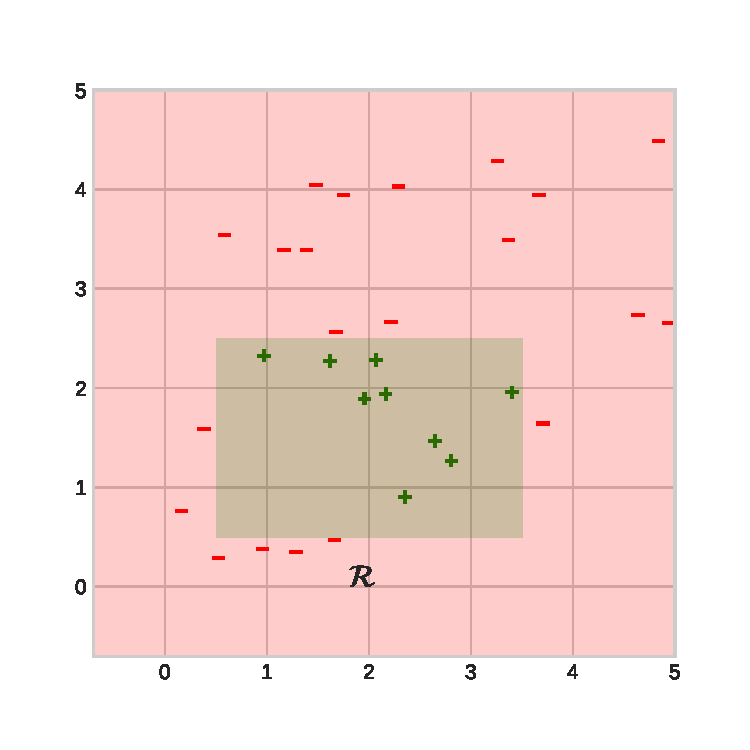
\includegraphics[width=8cm]{traget-and-sample.pdf}  
    \end{center}
    \caption{The target rectangle \(\rectangle\) along with a labeled sample of points}
    \label{fig:traget-and-sample}
\end{figure}

The player's goal is to find a hypothesis rectangle \(\rectangle^\prime\) that ``approximates'' \(\rectangle\) ``as closely as possible''. To measure the quality of this approximation, we will consider the region \(\rectangle\Delta\rectangle^\prime\) of points that \(\rectangle\) and \(\rectangle^\prime\) label differntly. More precisely, we will consider the probability \(\mathbb{P}(\rectangle\Delta\rectangle^\prime)\) of falling with this region according to \(\mathcal{D}\) and try to minimize this quantity.

Since \(\rectangle\) is unknown in practice, \(\rectangle^\prime\) is evaluated by sampling a number of points from \(\mathcal{D}\), labeling them using \(\rectangle^\prime\) and comparing to their true labels by asking the game. We then take the number of falsely labeled points devided by the total of chosen points as an estimation of \(\mathbb{P}(\rectangle\Delta\rectangle^\prime)\).
Note that this score is the same as \(1 - \mathrm{accuracy}\).

A simple strategy for the player is to sample a sufficiently large number \(m\) of points form \(\mathcal{D}\) and request their labels, then chose as hypothesis \(\rectangle^\prime\) the smallest rectangle containing all positive examples and no negative ones\footnote{Note that such at least one rectangle with this property is garenteed to exist, because \(\rectangle\) is one such a rectangle}. If all \(m\) points are negative, we chose \(\rectangle^\prime = \emptyset\). Figure~\ref{fig:traget-hypothesis-and-sample} ilustrates this strategy for one example, and Code~Snippet~\ref{lst:python-learning-rectangle} shows a python implementation.


\begin{figure}
    \begin{center}
        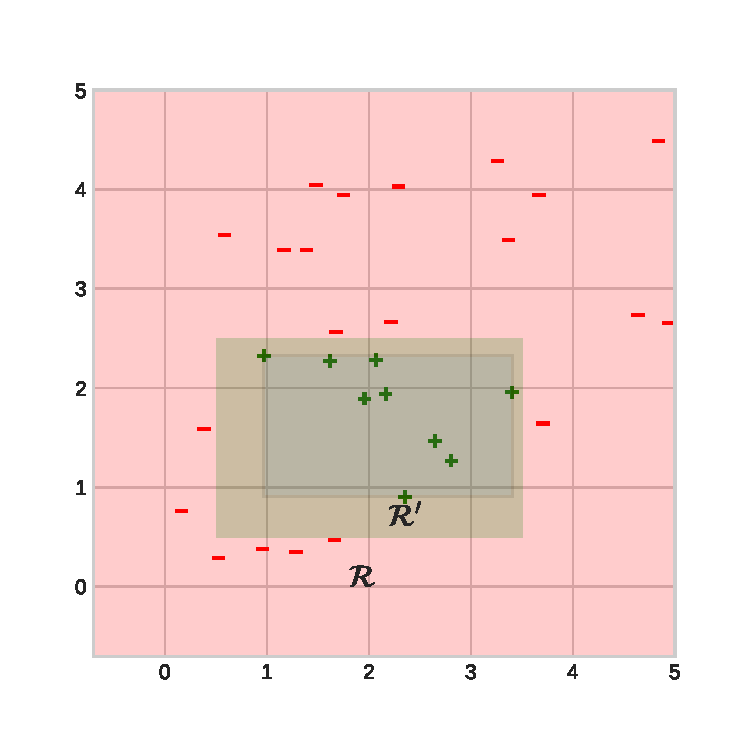
\includegraphics[width=8cm]{traget-hypothesis-and-sample.pdf}
    \end{center}
    \caption{The tightest fit rectangle for the example of Figure~\ref{fig:traget-and-sample}}
    \label{fig:traget-hypothesis-and-sample}
\end{figure}

\lstinputlisting[language=python, caption={A python implementation of the described strategy}, label={lst:python-learning-rectangle}, firstline=14, lastline=20]{../source/rectangle-learning.py}

We will now prove that this strategy works, more specifically, we will show the following theorem:

\begin{theorem}
    \ \\
    Let \(\mathcal{D}\) be a distribution over \(\reals^2\), \(\rectangle\) a rectangle, and \(\varepsilon, \delta>0\) be positive real numbers.
    There exisits an integer \(m\in\naturals\), such that the hypothesis rectangle \(\rectangle^\prime\) generated by \(m\) sampled points has with probability \(\ge 1 - \delta\) an error \(\le\varepsilon\).
\end{theorem}

\begin{proof}
    \ \\
    Consider a distribution \(\mathcal{D}\), a rectangle \(\rectangle = [a, b]\times[c, d]\), a hypothesis rectangle \(\rectangle^\prime = [a^\prime, b^\prime] \times [c^\prime, d^\prime]\) constructed using the startegy we described, and positive real numbers \(\varepsilon, \delta>0\).

    Note that \(\rectangle^\prime\) cannot have false positives. In fact, \(\rectangle^\prime\subset\rectangle\) and therefore \(\rectangle^\prime~\Delta\rectangle = \rectangle\backslash\rectangle^\prime\). 
    This region can be expressed as the union of four rectangles: 

    \[
        \begin{array}{ccc}
            \rectangle\backslash\rectangle^\prime = & [a, a^\prime] \times [c^\prime, d^\prime]& \cup\\
                & [a, b] \times [c, c^\prime] & \cup\\
                & [b^\prime, b] \times [c^\prime, d^\prime] & \cup\\
                & [a, b] \times [d, d^\prime]
        \end{array}
    \]
    We denote the union of four rectangles respectively by \(L, B, R, T\). It immediately follows that:
    \[
        \mathbb{P}(\rectangle\backslash\rectangle^\prime) = \mathbb{P}(L \cup B \cup R \cup T) \le \mathbb{P}(L) + \mathbb{P}(B) + \mathbb{P}(R) + \mathbb{P}(T)    
    \]
    
    Consequently, to show that \(\mathbb{P}(\rectangle\backslash\rectangle^\prime) \le \varepsilon\), it suffices to show that \(\mathbb{P}(X) \le \frac{\varepsilon}{4}\) for all \(X\in\{L, B, R, T\}\).

\end{proof}
    \section{A General Model}
\end{document}